\section{Experiments}
\label{sec:exp}
In this section, we conduct experiments on various real-world datasets. In our experiments, we use \textbf{NAP-[initial]} to denote the combination of NAP with another method, where \textbf{[initial]} represents the initial letter of the method's name (e.g., NAP-A for the combination with ASH). Specifically, we combine NAP with a series of common OOD detection methods, including ASH, DICE, Energy, KNN, MSP, and ReAct, denoted as NAP-A, NAP-D, NAP-E, NAP-K, NAP-M, and NAP-R, respectively. CIFAR-10, CIFAR-100, and ImageNet are used as ID datasets. For each combination of NAP with other methods, we use the approach described in Section~\ref{sec:how_to_find_w} to determine the optimal combination parameter \( w \). Detailed optimal \( w \) values for different experimental setups can be found in Appendix~\ref{appendix:w}. It's noted that the value of $\epsilon$ in our scoring functions is consistently set to $1.0$ for numerical stability. All experiments were conducted on an NVIDIA GeForce RTX 3090 GPU.

\subsection{Evaluation on CIFAR benchmarks}
\noindent \textbf{Implementation details.} In our experiments, consistent with recent studies~\cite{sun2021react, sun2022dice, djurisic2022extremely}, we utilized 10,000 test images from both CIFAR-10~\cite{krizhevsky2009cifar} and CIFAR-100~\cite{krizhevsky2009cifar} as ID data. To gauge the performance of the model, six widely-used OOD datasets were employed as benchmarks. These datasets include SVHN~\cite{netzer2011svhn}, Textures~\cite{cimpoi2014texture}, iSUN~\cite{xu2015isun}, LSUN-Crop~\cite{yu2015lsun}, LSUN-Resize~\cite{yu2015lsun}, and Places365~\cite{zhou2017places}. As for pre-trained model, we employed DenseNet~\cite{huang2017densely}, and we follow the training setting of DenseNet introduced in~\cite{sun2022dice}. 

\begin{table}[!b]
\centering
\caption{\textbf{Comparison with competitive post-hoc OOD detection method on CIFAR benchmarks.} All values are percentages and are averaged over 6 OOD test datasets.  Note: A. = Area Under the ROC Curve; F. = False Positive Rate at 95\% True Positive Rate. Methods include ASH~\cite{djurisic2022extremely}, DICE~\cite{sun2022dice}, Energy~\cite{liu2020energy}, KNN~\cite{sun2022knn}, MSP~\cite{hendrycks2016msp}, and ReAct~\cite{sun2021react}.\\}
\label{tab:cifar-avg}
% \tabcolsep=0.16cm
\scriptsize
\resizebox{\textwidth}{!}{
\begin{tabular}{@{}cc|c
c| c
c| c
c| c
c| c
c| c
c @{}}
\toprule
\textbf{Method}                      &    & ASH & \textbf{NAP-A} & DICE  & \textbf{NAP-D} & Energy & \textbf{NAP-E} & KNN   & \textbf{NAP-K} & MSP   & \textbf{NAP-M} & ReAct & \textbf{NAP-R} \\ \midrule
                                     & F.~$\downarrow$ & 15.05 & \textbf{11.14}    & 20.83 & \textbf{11.66} & 26.55  & \textbf{9.02}  & 16.12 & \textbf{7.79}  & 48.69 & \textbf{19.09} & 26.45 & \textbf{9.18}  \\
\multirow{-2}{*}{\textbf{CIFAR-10}}  & A.~$\uparrow$ & 96.91 & \textbf{97.48}    & 95.24 & \textbf{97.47} & 94.67  & \textbf{98.15} & 96.79 & \textbf{98.38} & 92.52 & \textbf{95.11} & 94.67 & \textbf{98.02} \\ \midrule
                                     & F.~$\downarrow$ & 41.40 & \textbf{35.40}    & 49.72 & \textbf{32.34}      & 68.45  & \textbf{32.61} & 44.91 & \textbf{33.63} & 80.13 & \textbf{48.20}      & 62.27 & \textbf{25.71} \\
\multirow{-2}{*}{\textbf{CIFAR-100}} & A.~$\uparrow$ & 90.02 & \textbf{91.21}    & 87.23 & \textbf{92.23}      & 81.19  & \textbf{92.84} & 86.58 & \textbf{91.54} & 74.36 & \textbf{88.45}      & 84.47 & \textbf{93.18} \\ \bottomrule
\end{tabular}
}
\end{table}

\noindent \textbf{Experimental results.} Table \ref{tab:cifar-avg} presents the comparison of NAP combined with other post hoc OOD detection methods on the CIFAR-10 and CIFAR-100 benchmarks. As shown in the table, our approach significantly enhances the performance of all methods on both CIFAR-10 and CIFAR-100 datasets. Notably, the maximum reductions in FPR95 on CIFAR-10 and CIFAR-100 are 66.03\% (NAP-E) and 58.71\% (NAP-R), respectively. Note that the table showcases the average performance across six OOD datasets; for complete performance details, please refer to Appendix~\ref{appendix:cifar}.



\begin{table}[!t]
% \tabcolsep=0.15cm
\scriptsize
\centering
\caption{\textbf{OOD detection results on ImageNet-1k~\cite{deng2009imagenet}.} All values are percentages. Methods include ASH~\cite{djurisic2022extremely}, DICE~\cite{sun2022dice}, Energy~\cite{liu2020energy}, KNN~\cite{sun2022knn}, MSP~\cite{hendrycks2016msp}, and ReAct~\cite{sun2021react}.\\ }
\label{tab:imagenet}
\resizebox{\textwidth}{!}{
\begin{tabular}{LcccccccccR}
\toprule
\multicolumn{1}{c}{\multirow{3}{*}{\textbf{Method}}} & \multicolumn{8}{c}{\textbf{OOD Datasets}}                                                                                                                                                                                                                                                             & \multicolumn{2}{c}{\multirow{2}{*}{\textbf{Average}}} \\ \cmidrule(lr){2-9}
\multicolumn{1}{c}{}                                 & \multicolumn{2}{c}{\textbf{iNaturalist}~\cite{van2018inaturalist}} & \multicolumn{2}{c}{\textbf{SUN}~\cite{xiao2010sun}} & \multicolumn{2}{c}{\textbf{Places}~\cite{zhou2017places}} & \multicolumn{2}{c}{\textbf{Textures}~\cite{cimpoi2014texture}} & \multicolumn{2}{c}{} \\ \cmidrule(l){10-11} 
\multicolumn{1}{c}{}                                 & FPR95~$\downarrow$          & AUROC~$\uparrow$                              & FPR95~$\downarrow$                              & AUROC~$\uparrow$                               & FPR95~$\downarrow$                              & AUROC~$\uparrow$                               & FPR95~$\downarrow$                              & AUROC~$\uparrow$                               & FPR95~$\downarrow$          & AUROC~$\uparrow$              \\ \midrule
ASH~\cite{djurisic2022extremely}                    & 31.46          & 94.28                              & 38.45                              & 91.61                              & 51.80                              & 87.56                              & 20.92                              & 95.07                              & 35.66          & 92.13                        \\
\rowcolor[HTML]{C0C0C0}
\textbf{NAP-A}                                       & \textbf{26.26}          & \textbf{95.10}                              & \textbf{32.89}                     & \textbf{92.77}                     & \textbf{48.69}                     & \textbf{87.92}                     & \textbf{11.60}                              & \textbf{97.32}                              & \textbf{29.86} & \textbf{93.28}                     \\ 
DICE~\cite{sun2022dice}                             & 43.09          & 90.83                              & 38.69                              & 90.46                              & 53.11                              & 85.81                              & 32.80                              & 91.30                              & 41.92          & 89.60                              \\
\rowcolor[HTML]{C0C0C0}
\textbf{NAP-D}                                       & \textbf{27.48}          &  \textbf{94.13}                             &  \textbf{36.14}                    &  \textbf{90.66}                    &  \textbf{51.84}                    &  \textbf{85.03}                    &   \textbf{9.02}                            &  \textbf{97.92}                             & \textbf{31.12} &  \textbf{91.94}                    \\ 
Energy~\cite{liu2020energy}                          & 59.50          & 88.91                              & 62.65                              & 84.50                              & 69.37                              & 81.19                              & 58.05                              & 85.03                              & 62.39          & 84.91                              \\
\rowcolor[HTML]{C0C0C0}
\textbf{NAP-E}                                       & \textbf{29.90}          & \textbf{94.47}                              & \textbf{39.69}                              & \textbf{90.46}                              & \textbf{55.17}                              & \textbf{85.15}                              & \textbf{11.74}                              & \textbf{97.28}                              & \textbf{34.12}          & \textbf{91.84}    \\ 
KNN~\cite{sun2022knn}                          & 85.91          & 72.67                              & 90.49                              & 65.39                              & 93.18                              & 60.08                              & 14.08                              & 96.98                              & 70.92          & 73.78                              \\
\rowcolor[HTML]{C0C0C0}
\textbf{NAP-K}                                       & \textbf{38.23}          & \textbf{89.80}                              & \textbf{56.55}                     & \textbf{80.01}                     & \textbf{70.89}                     & \textbf{71.35}                     & \textbf{7.02}                              & \textbf{98.39}                              & \textbf{43.17} & \textbf{84.89}                     \\ 
MSP~\cite{hendrycks2016msp}                          & 64.29          & 85.32                              & 77.02                              & 77.10                              & 79.23                              & 76.27                              & 73.51                              & 77.30                              & 73.51          & 79.00           \\
\rowcolor[HTML]{C0C0C0}
\textbf{NAP-M}                                       & \textbf{35.47}          & \textbf{92.53}                              & \textbf{51.19}                     & \textbf{86.51}                     & \textbf{63.77}                     & \textbf{80.61}                     & \textbf{15.14}                              &  \textbf{97.09}                             & \textbf{41.39} & \textbf{89.19}                     \\ 
ReAct~\cite{sun2021react}                           & 42.40          & 91.53                              & 47.69                              & 88.16                              & 51.56                              & 86.64                              & 38.42                              & 91.53                              & 45.02          & 89.47                              \\
\rowcolor[HTML]{C0C0C0}
\textbf{NAP-R}                                       & \textbf{24.58} & \textbf{95.55}                     & \textbf{38.47}                               & \textbf{91.12}                             & \textbf{53.32}                              & \textbf{86.24}                              & \textbf{9.57}                      & \textbf{97.60}                     & \textbf{31.49}          & \textbf{92.63}                     \\  \bottomrule
\end{tabular}
}
\end{table}


\subsection{Evaluation on ImageNet}
\label{sec:imagenet}
\noindent \textbf{Implementation details.} In real-world applications, models are confronted with high-resolution images spanning a diverse range of scenes and features. Evaluations on large-scale datasets can provide insights into the performance of models in practical deployments. Thus, in line with recent research~\cite{sun2021react, sun2022dice, djurisic2022extremely}, we conduct experiments with NAP on the expansive ImageNet-1k~\cite{deng2009imagenet} dataset in this study. Four dataset subsets, with all overlapping categories with ImageNet-1k eliminated, were employed as OOD benchmarks. These OOD datasets comprise Textures~\cite{cimpoi2014texture}, Places365~\cite{zhou2017places}, iNaturalist~\cite{van2018inaturalist}, and SUN~\cite{xiao2010sun}. We used MobileNetV2~\cite{sandler2018mobilenetv2} architecture, which pre-trained on ImageNet-1k~\cite{deng2009imagenet}. The architecture and parameters remain unchanged during the OOD detection stage.
% Parallel to the experiments conducted on the CIFAR~\cite{krizhevsky2009cifar} benchmarks, we experimented with three distinct implementations. For parameter settings, $w$ was set to $0.6$ for \textbf{NAP-E}, $0.8$ for \textbf{NAP-A}, and $0.8$ for \textbf{NAP-R}. 

\noindent \textbf{Experimental results.} Table \ref{tab:imagenet} shows the comparison results of NAP with other post-hoc OOD detection methods on the ImageNet-1k~\cite{deng2009imagenet} benchmark. As shown in the table, our approach significantly enhances the performance of all methods on the ImageNet-1k dataset~\cite{deng2009imagenet}. We have observed that our method brings significant performance improvements on the iNaturalist and Textures datasets, which is particularly notable. Intuitively, most of the pictures in the Textures~\cite{cimpoi2014texture} dataset are of a texture nature, so there is a small probability of obtaining a large response value. And while samples in iNaturalist have a relatively simple background, and the animals and plants in the foreground have certain semantic differences from the samples in ImageNet-1k, therefor, a sample in iNaturalist~\cite{van2018inaturalist} is not likely to trigger large response values. The reason why existing methods do not perform well on this dataset may be due to their focus on activation values after global pooling. We speculate that although texture pictures cannot cause large activation values, they can excite small-amplitude noise on the entire feature map. Since large response values tend to only appear in a small area on the feature map, after global pooling, ID samples and texture class samples are likely to obtain similar average activation values. This may compromise the separability of the two types of samples, causing existing work to perform poorly on such samples.

\subsection{Evaluation on Transformer}
Following the experimental setup described in Section~\ref{sec:imagenet}, we conduct experiments on the Vision Transformer~\cite{dosovitskiy2020image} (ViT-B/16) using ImageNet-1k as the ID dataset. Energy~\cite{liu2020energy} and MSP~\cite{hendrycks2016msp} were selected as baseline methodologies for this analysis. The study further explores the enhancement of these baseline methods through the integration of NAP, resulting in two variants: NAP-E and NAP-M. Comparative results detailed in Table~\ref{tab:vit} demonstrate that the NAP method substantially boosts the performance on Transformer architectures beyond the baselines, affirming the utility and versatility of NAP within such contexts.
\begin{table}[!h]
% \tabcolsep=0.15cm
\scriptsize
\centering
\caption{\textbf{OOD detection results on ViT-B/16 using ImageNet-1k as ID data.} All values are percentages. \\ }

\label{tab:vit}
\resizebox{\textwidth}{!}{
\begin{tabular}{LcccccccccR}
\toprule
\multicolumn{1}{c}{\multirow{3}{*}{\textbf{Method}}} & \multicolumn{8}{c}{\textbf{OOD Datasets}}                                                                                                                                                                                                                                                             & \multicolumn{2}{c}{\multirow{2}{*}{\textbf{Average}}}                   \\ \cmidrule(lr){2-9}
\multicolumn{1}{c}{}                                 & \multicolumn{2}{c}{\textbf{iNaturalist}~\cite{van2018inaturalist}}                                & \multicolumn{2}{c}{\textbf{SUN}~\cite{xiao2010sun}}                                        & \multicolumn{2}{c}{\textbf{Places}~\cite{zhou2017places}}                                     & \multicolumn{2}{c}{\textbf{Textures}~\cite{cimpoi2014texture}}                                   & \multicolumn{2}{c}{}                                                    \\ \cmidrule(l){10-11} 
\multicolumn{1}{c}{}                                 & FPR95~$\downarrow$          & AUROC~$\uparrow$                               & FPR95~$\downarrow$                               & AUROC~$\uparrow$                               & FPR95~$\downarrow$                              & AUROC~$\uparrow$                               & FPR95~$\downarrow$                              & AUROC~$\uparrow$                               & FPR95~$\downarrow$          & AUROC~$\uparrow$                               \\ \midrule
Energy~\cite{liu2020energy}                           & \multicolumn{1}{c}{64.08}          & 79.24                              & 72.77                              & 70.25                              & 74.30                              & 68.44                              & 58.46                              & 79.30                              & \multicolumn{1}{c}{67.40}          & 74.31                              \\
\rowcolor[HTML]{C0C0C0}
\textbf{NAP-E}                                & \textbf{60.97}  & \textbf{80.77}                     & \textbf{64.05}                               & \textbf{77.34}                              & \textbf{69.34}                               & \textbf{73.30}                              & \textbf{45.04}                       & \textbf{86.93}                     & \textbf{59.85} & \textbf{79.58}                     \\  
MSP~\cite{hendrycks2016msp}                            & \multicolumn{1}{c}{51.47}          & 88.16                              & 66.53                              & 80.93                              & 68.65                              & 80.38                              & 60.21                              & 82.99                              & \multicolumn{1}{c}{61.72}          & 83.12                              \\
\rowcolor[HTML]{C0C0C0}
\textbf{NAP-M}            &      \textbf{47.09}    &      \textbf{88.23}        & \textbf{59.45}                              &      \textbf{82.78}    & \textbf{63.38}             & \textbf{80.48}                              &      \textbf{47.70}    &      \textbf{87.93}        &      \textbf{54.40}                              &      \textbf{84.85}    \\ \bottomrule
\end{tabular}
}
\end{table}

\noindent\textbf{Discussion.} We compare only with MSP~\cite{hendrycks2016msp} and Energy~\cite{liu2020energy} because methods such as ASH~\cite{djurisic2022extremely} and ReAct~\cite{sun2021react} are specifically designed for CNNs and fail completely when applied to ViT. For fairness, we do not include these methods in our comparison.




\subsection{Does NAP work across all network layers?}


\label{sec:does}
To assess the efficacy of the NAP across various layers within the DenseNet architecture, we conduct a detailed examination of activation distributions utilizing the CIFAR-10~\cite{krizhevsky2009cifar} and Places365 datasets~\cite{zhou2017places}. Analysis focused on four pivotal points within the network: post-first convolutional layer, pre-pooling in the first and second transition blocks, and immediately preceding the final global pooling layer.
Selected instances from the empirical findings are illustrated in Selected examples from our tests are shown in Figure~\ref{fig:max-mean}, with more detailed visuals in the Appendix~\ref{appendix:layer}. From these figures, it's clear that the deeper the layer, the easier it is to tell apart ID and OOD samples based on the maximum and average activation values. 
In the network's early layers, neurons pick up basic features common to both ID and OOD samples, which explains why the lines cross in Figures~\ref{fig:t1} and~\ref{fig:t2}. Moving to deeper layers, neurons start capturing more complex, meaningful features. As seen in Figures~\ref{fig:t3} and~\ref{fig:t4}, ID samples with specific meanings trigger larger responses. This indicates that NAP works best closer to the end of the network, especially before the global pooling layer, highlighting its value in making models more reliable for OOD detection.

\begin{figure}[h]
  \centering
  \begin{subfigure}{0.24\linewidth}
    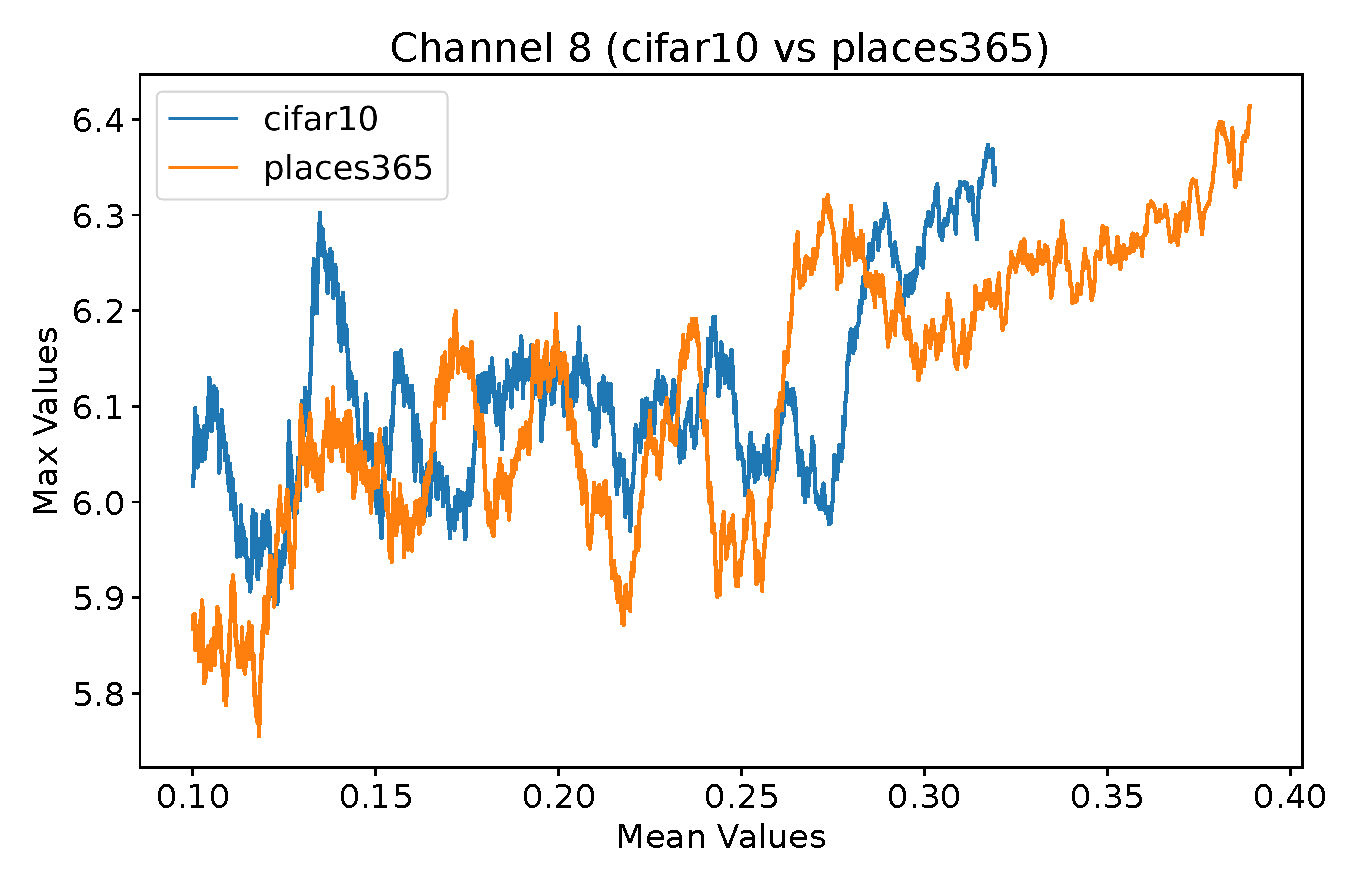
\includegraphics[width=0.99\linewidth]{eps/t0-channel_8.eps}
    \caption{After conv layer 1}
    \label{fig:t1}
  \end{subfigure}
  \hfill
  \begin{subfigure}{0.24\linewidth}
    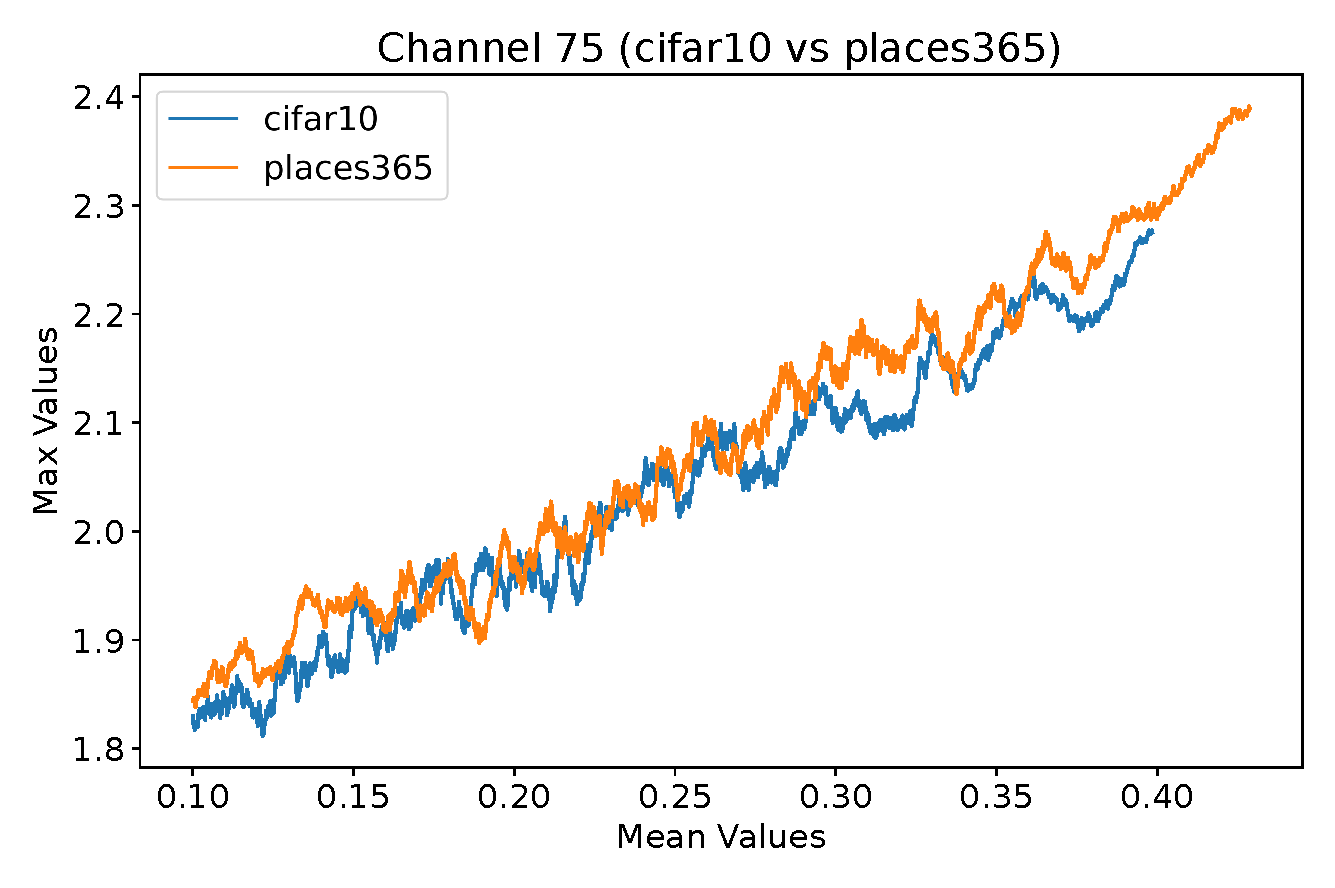
\includegraphics[width=0.99\linewidth]{eps/t1-channel_75.eps}
    \caption{In Trans Block 1}
    \label{fig:t2}
  \end{subfigure}
  \hfill
  \begin{subfigure}{0.24\linewidth}
    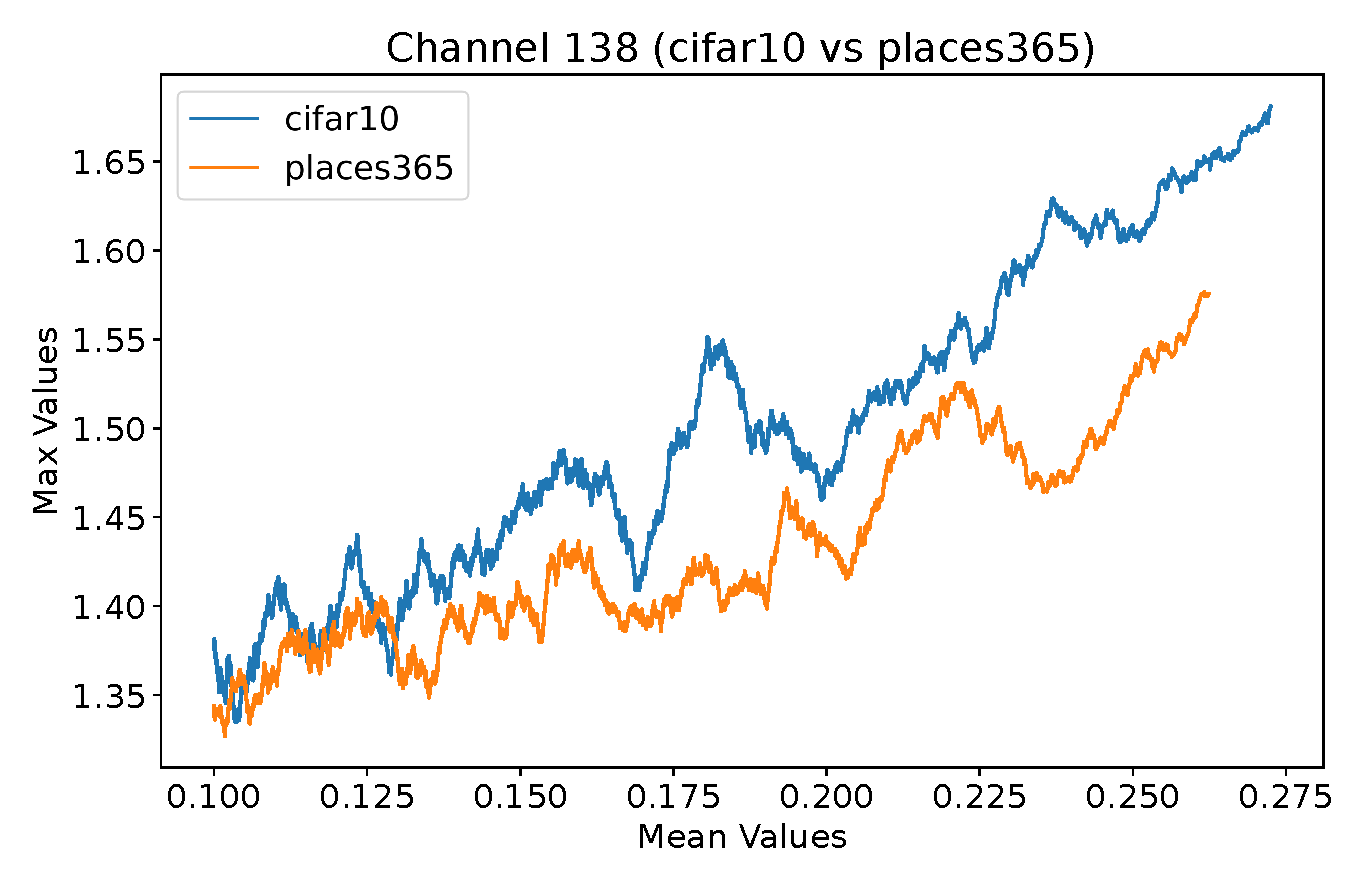
\includegraphics[width=0.99\linewidth]{eps/t2-channel_138.eps}
    \caption{In Trans Block 2}
    \label{fig:t3}
  \end{subfigure}
  \hfill
  \begin{subfigure}{0.24\linewidth}
    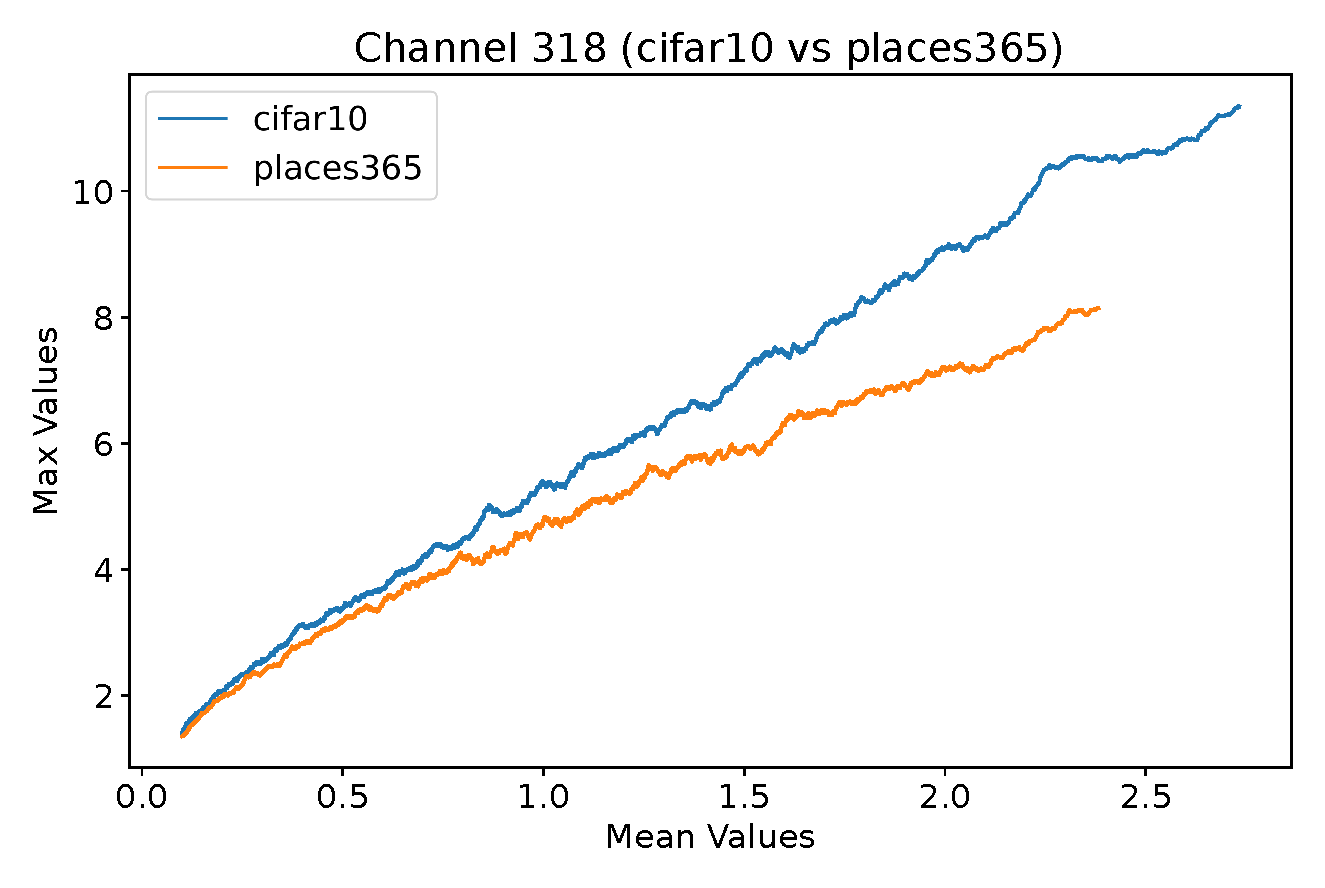
\includegraphics[width=0.99\linewidth]{eps/t3-channel_318.eps}
    \caption{Before Pooling}
    \label{fig:t4}
  \end{subfigure}
  \caption{\textbf{Activation distribution at different positions within the DenseNet architecture~\cite{huang2017densely} applied to CIFAR-10~\cite{krizhevsky2009cifar} and Places365 datasets~\cite{zhou2017places}.} For this analysis, four specific locations within the network were chosen: (a) after the first convolution layer, (b) just before the pooling operation in the first transition block, (c) just before the pooling operation in the second transition block, and (d) right before the final global pooling layer. It is observed that with increasing depth, the separability between ID and OOD samples becomes more pronounced in the two-dimensional space defined by the maximum and average activation values.}
  \label{fig:max-mean}
  % \vspace{-15pt}
\end{figure}